\section{2: VLAN}
Virtual Local Area Networks (VLANs) are a way to logically segment a single physical network into multiple virtual networks. VLANs allow network administrators to group devices and users based on their requirements, improving network performance, security, and management. By creating separate broadcast domains, VLANs reduce unnecessary traffic and improve overall efficiency. VLANs are widely used in enterprise networks, data centers, and other environments where network segmentation is required.
You have two switches (Switch1 and Switch2) and six hosts (PC1, PC2, PC3, PC4, PC5, and PC6) that need to be configured for three VLANs (VLAN10, VLAN20, and VLAN30). The configuration should be as follows:

\subsection{Intra-VLAN Ping}

\begin{enumerate}[label=\Roman*.]
    \item Configure the switches (Switch1 and Switch2) to support the three VLANs (VLAN10, VLAN20, and VLAN30).
    \item Configure the PCs to be part of their respective VLANs:
    \begin{itemize}
        \item VLAN10: PC1, PC4
        \item VLAN20: PC2, PC5
        \item VLAN30: PC3, PC6
    \end{itemize}
\end{enumerate}

In your report please explain your code and the configuration steps.

\begin{enumerate}[label=\Roman*.]
    \setcounter{enumi}{2}
    \item Write a script or code to perform the following ping tests
    \begin{itemize}
        \item PC1 pings PC4 (VLAN10)
        \item PC3 pings PC6 (VLAN30)
    \end{itemize}
\end{enumerate}
\begin{qsolve}
    \begin{qsolve}[]
        the network is shown in figure 18.
        \begin{figure}[H]
            \centering
            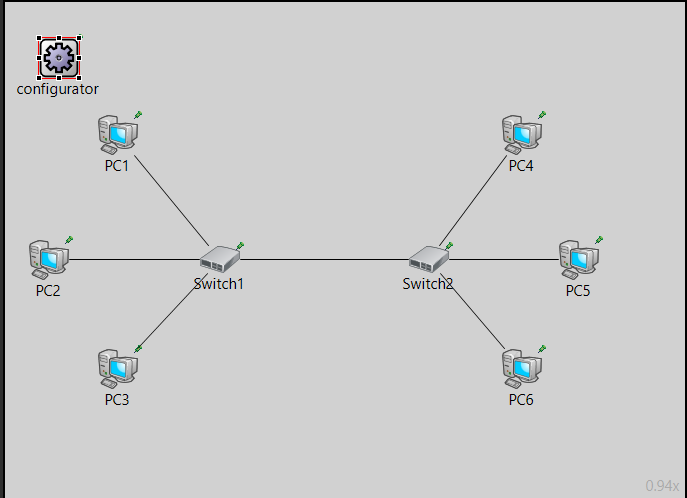
\includegraphics[width=0.7\textwidth]{Q2_1network.png}
            \caption{Network diagram}
        \end{figure}
        \splitqsolve[\splitqsolve]
        you can see the .NED file in figure 19. 
        \begin{figure}[H]
            \centering
            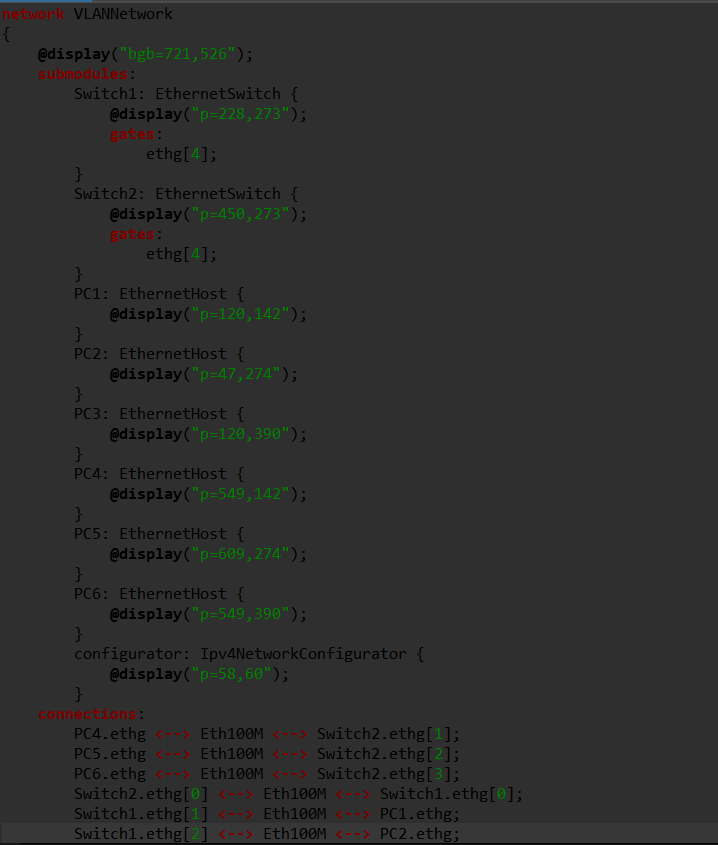
\includegraphics[width=0.7\textwidth]{Q2_1ned.png}
            \caption{NED file}
        \end{figure}
        The network consists of the following components:
        \begin{enumerate}
            \item Two Ethernet switches (Switch1 and Switch2) to support the VLANs.
            \item Six Ethernet hosts (PC1, PC2, PC3, PC4, PC5, and PC6) representing the devices connected to the VLANs.
            \item An IPv4 network configurator (configurator) to handle the IP address assignment and other network configuration tasks.
        \end{enumerate}
        This network setup allows for the simulation of VLAN configurations, traffic management, inter-VLAN and intra-VLAN communication through the switches.

        the functionality of the network is handled using a .XML file and a .ini file. the .xml code snippet which is shown in figure 20 configures the network interfaces of six hosts  with specific IP addresses and subnet masks. Each <interface> tag specifies the network configuration for a particular host.this configuration assigns unique IP addresses and a common subnet mask to each of the six PCs, effectively organizing them into three different subnets:
        \begin{enumerate}
            \item Subnet 10.0.10.0/24 for PC1 and PC4.
            \item Subnet 10.0.20.0/24 for PC2 and PC5.
            \item Subnet 10.0.30.0/24 for PC3 and PC6.
        \end{enumerate}
        \splitqsolve[\splitqsolve]
        on the other hand the .ini file does all the functionallity as all parts are from inet framework ther is no need for a .cc file.the .ini file which is shown in figure 21 sets up a VLAN network simulation with specific VLAN IDs for each PC's Ethernet interface, configures which PCs will communicate with each other, and specifies an external XML file for detailed network configuration. The simulation is limited to 10 seconds in duration.
        \begin{figure}[H]
            \centering
            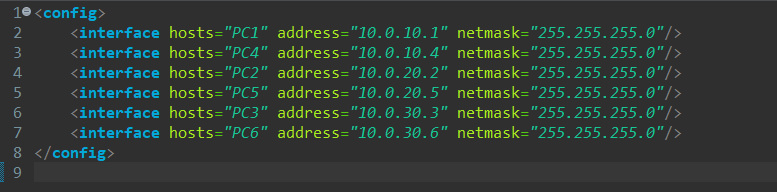
\includegraphics[width=0.7\textwidth]{Q2_1xml.png}
            \caption{XML file}
        \end{figure}
        \begin{figure}[H]
            \centering
            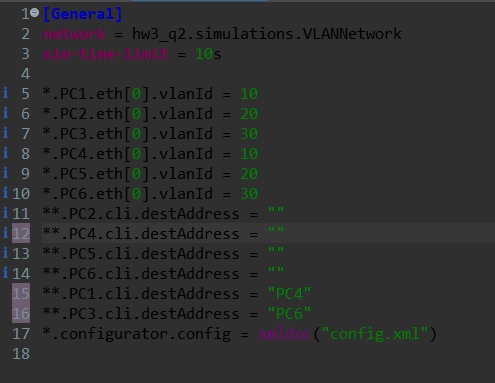
\includegraphics[width=0.7\textwidth]{Q2_1ini.png}
            \caption{INI file}
        \end{figure}
        to show that PC1 can ping PC4 and PC3 can ping PC6 i recorded a video which is attached with files that have been sent. the name of the video is ping1.
    \end{qsolve}
\end{qsolve}
\subsection{Inter-VLAN Ping}
\begin{enumerate}[label=\Roman*.]
    \item Configure the switches (Switch1 and Switch2) to support inter-VLAN communication (e.g., using a trunk link).
    \item Write a script or code to perform the following ping tests:
    \begin{itemize}
        \item PC1 (VLAN10) pings PC2 (VLAN20)
        \item PC4 (VLAN10) pings PC6 (VLAN30)
    \end{itemize}
\end{enumerate}

Please explain your code and the configuration steps, including how inter-VLAN communication is achieved.
\begin{qsolve}
    \begin{qsolve}[]
        the network topology and .NED and XML file is as the same as before. but the .ini file is changed so the network can support inter-VLAN. the .ini file is shown in figure 22.
        \begin{figure}[H]
            \centering
            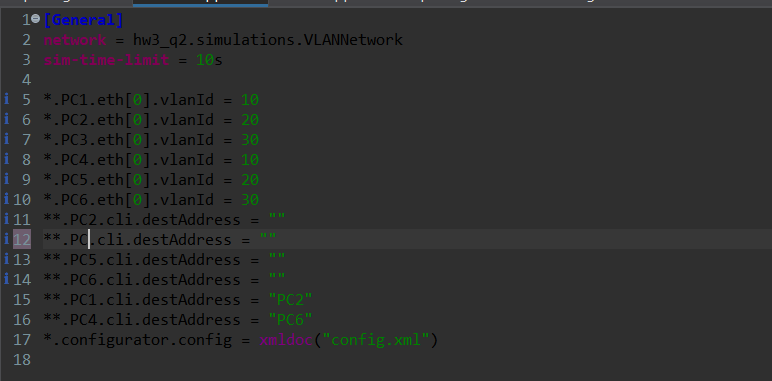
\includegraphics[width=0.7\textwidth]{Q2_2ini.png}
            \caption{INI file}
        \end{figure}
        to show that PC1 can ping PC2 and PC4 can ping PC6 i recorded a video which is attached with files that have been sent. the name of the video is ping2.
    \end{qsolve}
\end{qsolve}